Para analizar la conexión en serie, se utilizarán cinco compuertas con las siguientes característicsa:
\begin{itemize}
    \item $W_{n_2} = 2\cdot W_{n_1}$
    \item $W_{p_2} = 2\cdot W_{p_1}$
    \item $W_{n_3} = 4\cdot W_{n_1}$
    \item $W_{p_3} = 4\cdot W_{p_1}$
    \item $W_{n_4} = 8\cdot W_{n_1}$
    \item $W_{p_4} = 8\cdot W_{p_1}$
    \item $W_{n_5} = 16\cdot W_{n_1}$
    \item $W_{p_5} = 16\cdot W_{p_1}$
\end{itemize}

Es esperable que los tiempos de propagación aumenten a medida que se agregan compuertas en serie.
Sin embargo no se dió así la simulación.
\begin{figure}[H]
        \subfigure[Tiempo de LOW a HIGH]{
            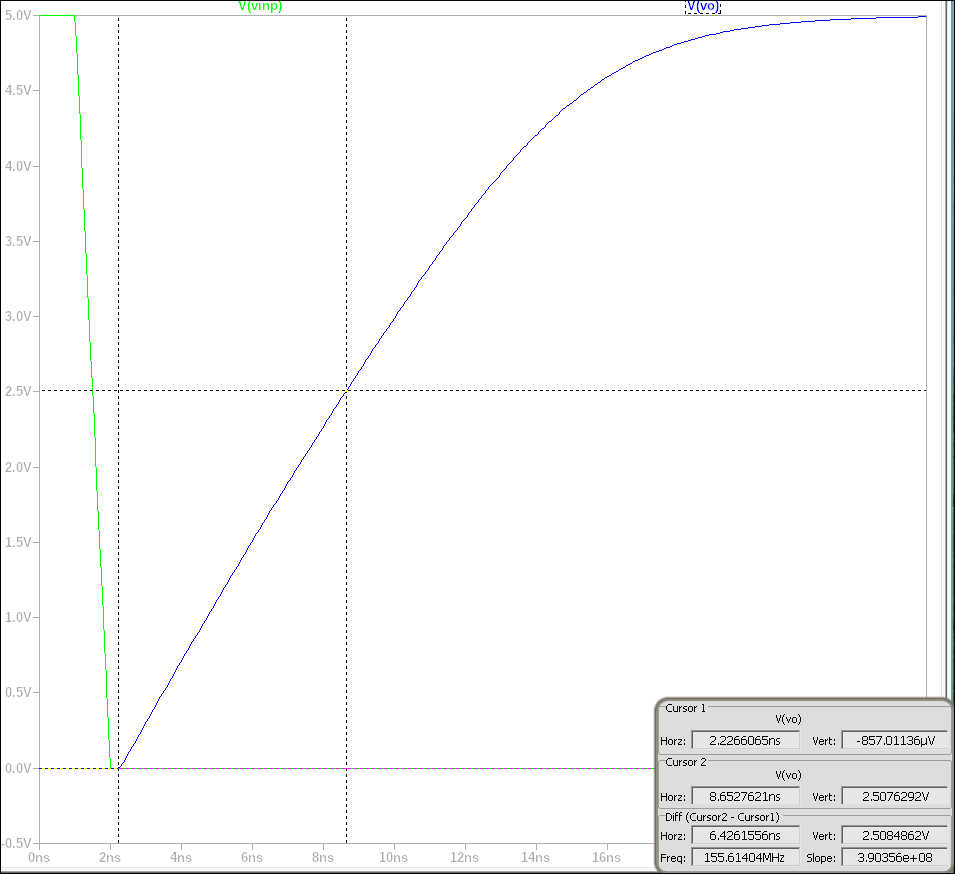
\includegraphics[width=.48\linewidth]{Imagenes/tL2HSerie.png}
            \label{subfig:tL2Hserie}
        }\hfill
        \subfigure[Tiempo de HIGH a LOW]{
            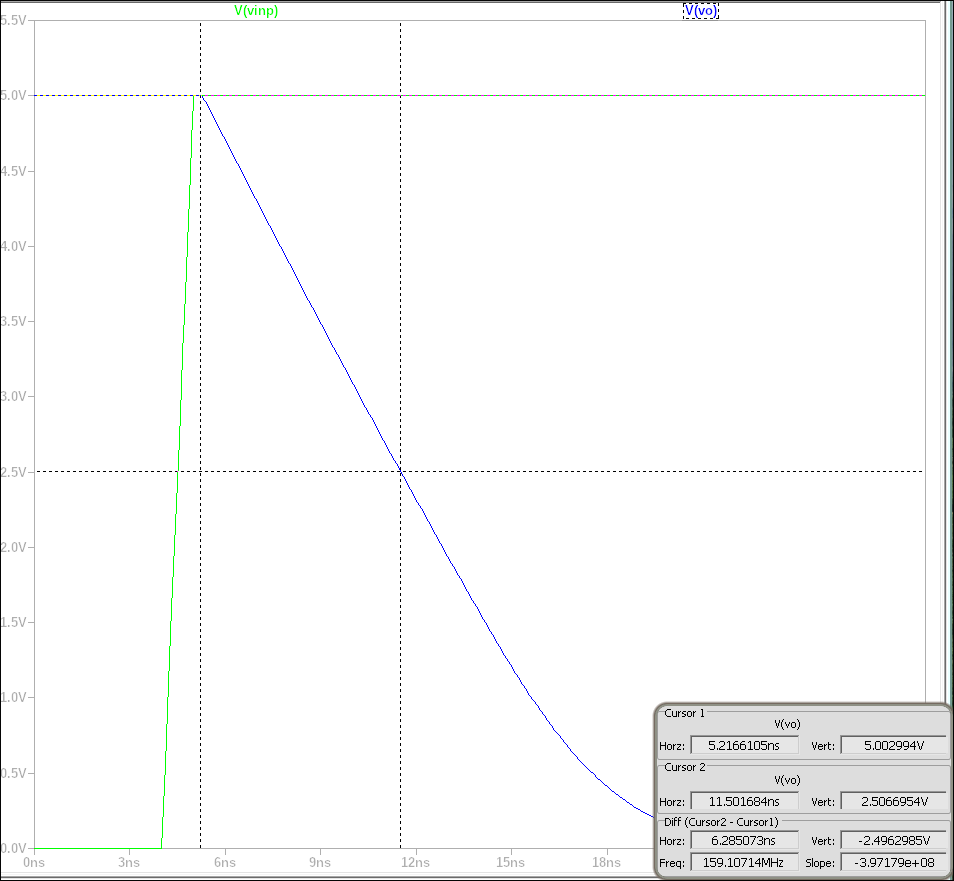
\includegraphics[width=.48\linewidth]{Imagenes/tH2LSerie.png}
            \label{subfig:tH2Lserie}
        }
        \caption{Tiempos de propagación para la compuerta NOT}
        \label{fig: tiempos_propagacionSerie}
\end{figure}
Esto se debe a que los anchos de las compuertas son diferentes entre si, donde la compuerta de mayor ancho se encuentra a la salida junto al capacitor.
Por eso el tiempo de propagación LOW to HIGH es de $t_{LtoH} = 6.43ns$ y el tiempo de propagación HIGH to LOW es de $t_{HtoL} = 6.28ns$. 
Los tiempos se mantuvieron cercanos entre sí debido a que los anchos de las compuertas mantuvieron la proporción de $\frac{\beta_n}{\beta_p}$.
